\documentclass[a4paper]{article}

%% Language and font encodings
\usepackage[english]{babel}
\usepackage[utf8x]{inputenc}
\usepackage[T1]{fontenc}

%% Sets page size and margins
\usepackage[a4paper,top=3cm,bottom=2cm,left=3cm,right=3cm,marginparwidth=1.75cm]{geometry}

%% Useful packages
\usepackage{amsmath}
\usepackage{graphicx}
\usepackage[colorinlistoftodos]{todonotes}
\usepackage[colorlinks=true, allcolors=blue]{hyperref}
\usepackage{framed}


\title{Computing for Medicine \\ \Large Project 5: Disease data capture using web technologies}
\author{}
\date{}

\begin{document}

\newcommand{\error}[1]{\textcolor{red}{#1}}

\maketitle

\section{PhenoTips and the Human PhenoType Ontology (HPO)}

The PhenoTips web application~\cite{phenotips} is used to collect and analyze patient information, including phenotypic information: \url{https://phenotips.org/}. PhenoTips is an open source software tool for collecting and analysing phenotypic information for patients with genetic disorders. The user interface closely mirrors clinician workflows so as to facilitate the recording of observations made during the patient encounter. This easy-to-use front-end, compatible with any device that runs a Web browser, is coupled with a standardized database back-end. 

PhenoTips  uses the Human Phenotype Ontology (HPO)~\cite{hpo} to name and classify phenotypic information: \url{http://human-phenotype-ontology.github.io/}. The HPO is a hierarchical representation of phenotypes (signs and symptoms, especially relevant for genetic diseases). These phenotypes are organized using an is-a relationship, from very general ("Phenotypic abnormality") to more specific ("abnormality of the hand") to very specific ("2-3 finger cutaneous syndactyly"). Overall the HPO contains $>12,000$ phenotypic terms, most of which are linked to relevant genetic disorders (OMIM database).  

\section{Part 0: Explore PhenoTips}

To begin, visit the PhenoTips playground (\url{https://playground.phenotips.org/}) and use the PhenoTips tool.  This instance of PhenoTips is publicly accessible and can be used without registering an account. Play with PhenoTips by creating new patient records and searching for existing patient records.  As you examine the records, pay special attention to the phenotypic information recorded for each patient.

\section{Part 1: Use the PhentoTips API}

In your first task for this project, you interacted with the PhenoTips website using a web browser.  Now, you will perform some of the same tasks, and others, using a Python program.

\subsection{PhenoTips API}

The developers of the PhenoTips web application have provided an API, which allows software developers to write programs that interact with PhenoTips.  Documentation and examples of using the PhenoTips API are posted here:\\

\url{https://phenotips.org/DevGuide/RESTfulAPI#HBasicexamplesusingaRESTclient}\\

Using the PhenoTips API, we can write code to retrieve a particular patient record or  all patient records from an instance of PhenoTips.  We can also make changes to patient records, add new patient records, and even delete patient records.

The data retrieved from PhenoTips is returned in a JSON format that is described here:\\

\url{https://phenotips.org/DevGuide/JSONExport}

\subsection{Your Tasks}
In \texttt{phenotips\_project.py}, there are three complete functions.  Read those functions, along with the PhenoTips API documentation, to gain a better understanding of how to write code that interacts with PhenoTips.  Next, complete the bodies of the following three functions:
\begin{itemize}
\item \texttt{get\_patients\_range}
\item \texttt{delete\_patient}
\item \texttt{get\_phenotypic\_info}
\end{itemize}

To test your code, use the example function calls in the main block.  You can also use the PhenoTips website search functionality to check whether your code performed as expected.

\section{Part 2: Human Phenotype Ontology (HPO)}

The Human Phenotype Ontology (\url{http://human-phenotype-ontology.github.io/}) is a classification of human phenotypic abnormalities observed in human disease.  The HPO has a hierarchical organization  with four main subcategories: \textit{mortality/aging}, \textit{phenotypic abnormality}, \textit{clinic modifier}, and 
\textit{mode of inheritance}.  Figure~\ref{four} shows this hierarchy, with the name of each category and its unique identifier. In this project, you will work only with the subcategory \textit{phenotypic abnormality}.

\begin{center}
\begin{figure}[h]
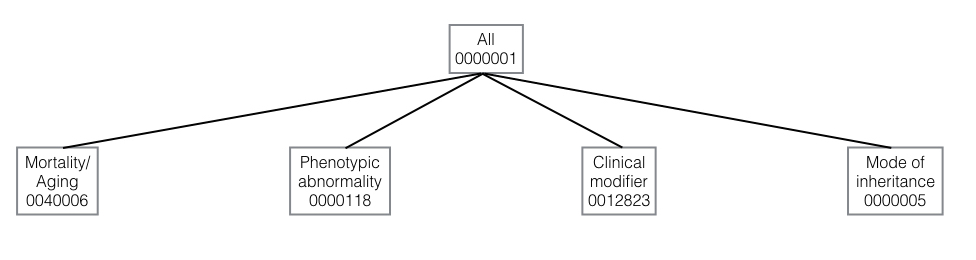
\includegraphics[width=5in]{ontology_four_categories.jpeg}
\caption{HPO's four subcategories}
\label{four}
\end{figure}
\end{center}

Figure~\ref{abnormalities} shows part of the HPO \textit{phenotypic abnormality} ontology.  Each phenotypic abnormality has a name and a unique numeric identifier.  The root of the hierarchy has ID 0000118 and 23 subcategories, including the three that are shown: Abnormality of the ear (0040006), Abnormality of the breast (0000769), and Abnormality of the voice (0001608).  Each of those phenotypic features may have subcategories as well, those subcategories may have subcategories, and so on.  
\begin{center}
\begin{figure}[h]
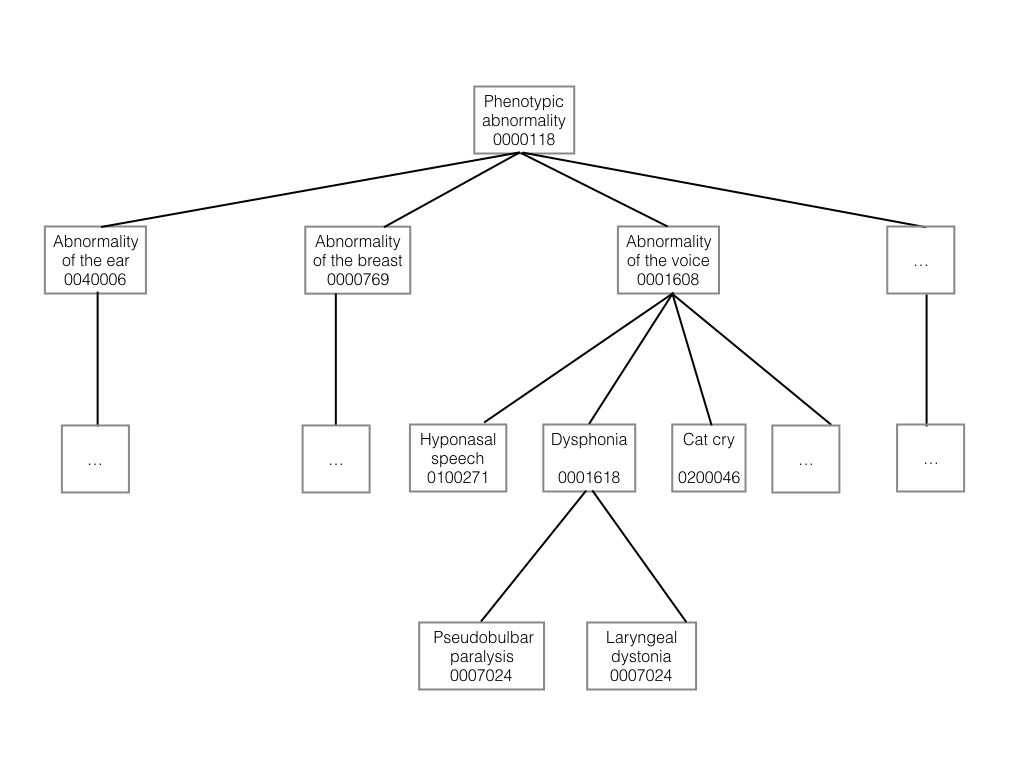
\includegraphics[width=6in]{ontology_img.jpeg}
\caption{Part of the phenotypic abnormality ontology}
\label{abnormalities}
\end{figure}
\end{center}

For each phenotypic abnormality, we will use a level number to describe its distance from the root.  For example, Abnormality of the voice, is at level 1, Hyponasal speech is at level 2, and Laryngeal dystonia is at level 3.

As part of the project files, we included the HPO file, \texttt{hp.obo} (accessed from the HPO website on 11 January 2017).  We also provided a Python program \texttt{ontology\_parser.py}, which reads and parses the HPO file, and produces two dictionaries containing information about the ontology:

\begin{itemize}
\item \texttt{pid\_to\_name}: each key is an ID for a phenotypic feature and each value is its name
\item \texttt{pid\_to\_parents}: each key is an ID for a phenotypic feature and each value is a list of its parent IDs
\end{itemize}

\subsection{Your tasks}

Starter code file \texttt{ontology\_explorer.py} contains several incomplete functions.  Your task is to complete these functions:
\begin{itemize}
\item \verb|get_single_path|
\item \verb|get_ids_at_level|
\item \verb|get_all_paths|
\item \verb|get_all_paths_to_level| \end{itemize}

\noindent Here are a few tips:
\begin{itemize}
\item Spend time thinking about the algorithms, before starting to write code.  
\item Trace examples on paper and use the debugger.
\item If your functions get long or can be divided into parts, consider writing helper functions to simplify your code.
\item As you implement each function, call on the examples from the main block to test your work.  Add example calls of your as well.
\item \verb|get_all_paths| and \verb|get_all_paths_to_level| are very similar.  Focus on getting one of those two functions working, before working on the other.
\end{itemize}

\newpage 
\section{Part 3: Q \& A}

In a file named \texttt{project5.txt}, answer the  questions below.  For some questions, you may find it helpful to write some code or call on your existing functions to find the answer.  For others, no programming is needed.

\begin{enumerate}
\item Instead of using \verb|get_all_paths|, we can use
\verb|get_all_paths_to_level| to find all paths to the root. Describe which arguments to pass to \verb|get_all_paths_to_level| to achieve this.
\item In HPO, what is the maximum number of parents that any phenotypic feature has?  Give the name and ID of one phenotypic feature that has the maximum number of parents.
\item In HPO, what is the maximum level (distance from the root) of any feature in the ontology?  Give the name and ID of one phenotypic feature at that level.
\end{enumerate}

\bibliography{project}{}
\bibliographystyle{plain}

\end{document}

